%%%%%%%%%%%%%%%%%%%%%%%%%%%%%%%%%%%%%%%%%%%%%%%%%%%%%%%%%%%%%%%%%%%%%%%%
%DIF LATEXDIFF DIFFERENCE FILE
%DIF DEL MercuryNumerical-oldtmp-47694.tex   Tue Apr 24 13:24:54 2018
%DIF ADD MercuryNumerical.tex                Tue Apr 24 13:12:08 2018
%    INSTITUTE OF PHYSICS PUBLISHING                                   %
%                                                                      %
%   `Preparing an article for publication in an Institute of Physics   %
%    Publishing journal using LaTeX'                                   %
%                                                                      %
%    LaTeX source code `ioplau2e.tex' used to generate `author         %
%    guidelines', the documentation explaining and demonstrating use   %
%    of the Institute of Physics Publishing LaTeX preprint files       %
%    `iopart.cls, iopart12.clo and iopart10.clo'.                      %
%                                                                      %
%    `ioplau2e.tex' itself uses LaTeX with `iopart.cls'                %
%                                                                      %
%%%%%%%%%%%%%%%%%%%%%%%%%%%%%%%%%%
%
%
% First we have a character check
%
% ! exclamation mark    " double quote
% # hash                ` opening quote (grave)
% & ampersand           ' closing quote (acute)
% $ dollar              % percent
% ( open parenthesis    ) close paren.
% - hyphen              = equals sign
% | vertical bar        ~ tilde
% @ at sign             _ underscore
% { open curly brace    } close curly
% [ open square         ] close square bracket
% + plus sign           ; semi-colon
% * asterisk            : colon
% < open angle bracket  > close angle
% , comma               . full stop
% ? question mark       / forward slash
% \ backslash           ^ circumflex
%
% ABCDEFGHIJKLMNOPQRSTUVWXYZ
% abcdefghijklmnopqrstuvwxyz
% 1234567890
%
%%%%%%%%%%%%%%%%%%%%%%%%%%%%%%%%%%%%%%%%%%%%%%%%%%%%%%%%%%%%%%%%%%%
%
\documentclass[12pt,ngerman,american]{iopart}
\newcommand{\gguide}{{\it Preparing graphics for IOP Publishing journals}}
%Uncomment next line if AMS fonts required
%\usepackage{iopams}

\usepackage[utf8]{inputenc}         % this is needed for Umlaute
\usepackage[main=american]{babel} % this is needed for Umlaute
\usepackage[T1]{fontenc}            % this is needed for correct output of umlauts in pdf
\usepackage{cite}



\usepackage[dvipsnames]{xcolor}         % Enabling colors by their 'svgnames'
\usepackage[%
  unicode=false,%
  pdftitle={A primer to numerical simulations: The perihelion motion of Mercury},%
  pdfauthor={C. K\"orber, I. Hammer, J.-L. Wynen, J. Heuer, C. M\"uller and C. Hanhart},%
  pdfkeywords={Numerical Simulations, Teaching, Perihelion Motion of Mercury, General Relativity},%
  pdfsubject={A primer with the goal to teach general concepts of numerical simulations to high school students.  The specific example is the perihelion motion of Mercury due to General Relativity.},   % subject of the document
  colorlinks=true,        % true: colored links
  linkcolor=OliveGreen,          % color of internal links (change box color with linkbordercolor)
  citecolor=magenta,        % color of links to bibliography
  filecolor=YellowGreen,      % color of file links
  urlcolor=blue           % color of external links
]{hyperref}
\usepackage[space=true]{accsupp}
% requires the latest version of package accsupp
\newcommand{\copyablespace}{\BeginAccSupp{method=hex,unicode,ActualText=00A0}\ \EndAccSupp{}}


%%%%%%%%%%%%%%%%%%%%%%%%%%%%%%%%%%%%%%%%%%%%%%%%%%%%%%%%%%%%%%%%%%%
% Custom
%%%%%%%%%%%%%%%%%%%%%%%%%%%%%%%%%%%%%%%%%%%%%%%%%%%%%%%%%%%%%%%%%%%

\usepackage{textcomp,gensymb}       % \degree

\usepackage[autostyle=true]{csquotes}            % Define quotation style
\MakeOuterQuote{"}                               % Text wrapped in "..." is recognized as a quotation

\usepackage{amssymb}                  % Math stuff
\usepackage{graphicx}                 % Import Pictures + PDFs
\usepackage{listings}                 % Code listings  See: https://en.wikibooks.org/wiki/LaTeX/Source_Code_Listings

\usepackage{subcaption} % subfigures


%%%%%%%%%%%%%%%%%%%%%%%%%%%%%%%%%%%%%%%%%%%%%%%%%%%%%%%%%%%%%%%%%%%
% Definitions
%%%%%%%%%%%%%%%%%%%%%%%%%%%%%%%%%%%%%%%%%%%%%%%%%%%%%%%%%%%%%%%%%%%
\definecolor{fzjblue}{HTML}{005B81}
\definecolor{light-gray}{gray}{0.97}
\definecolor{semilight-gray}{gray}{0.67}
\definecolor{mygreen}{rgb}{0,0.6,0}

% Custom code listings environment
\lstset{
  language=Python,
  backgroundcolor=\color{light-gray},   % choose the background color; you must add \usepackage{color} or \usepackage{xcolor}
  basicstyle=\linespread{1}\footnotesize\ttfamily,        % the size of the fonts that are used for the code
  commentstyle=\color{mygreen},
  frame=single,
  keywordstyle=\color{blue},       % keyword style
  tabsize=4,	                   % sets default tabsize to 2 spaces
  showtabs=false,
  rulecolor=\color{black},
  columns=fullflexible,
  literate={\ }{{\copyablespace}}1
}

\usepackage{tikz}
\usetikzlibrary{shapes.geometric, arrows}
%
\tikzstyle{startstop} = [
	rectangle,
	rounded corners,
	minimum width=3cm,
	minimum height=1cm,
	text width=4.5cm,
	text centered,
	draw=black,
	fill=green!30
]

\tikzstyle{process} = [
	rectangle,
	minimum width=3cm,
	minimum height=1cm,
	text width=4.5cm,
	text centered,
	draw=black,
	fill=blue!25
]
\tikzstyle{decision} = [
	diamond,
	minimum width=4.5cm,
	minimum height=1cm,
	text width=1.7cm,
	text centered,
	draw=black,
	fill=red!30
]
\tikzstyle{arrow} = [thick,->,>=stealth]

%%%%%%%%%%%%%%%%%%%%%%%%%%%%%%%%%%%%%%%%%%%%%%%%%%%%%%%%%%%%%%%%%%%
% Commands
%%%%%%%%%%%%%%%%%%%%%%%%%%%%%%%%%%%%%%%%%%%%%%%%%%%%%%%%%%%%%%%%%%%
\newcommand{\python}[0]{\texttt{Python}}
\newcommand{\vpython}[0]{\texttt{VPython}}
\newcommand{\abs}[1]{\left\vert #1 \right\vert}
\newcommand{\code}[1]{{\scriptsize\colorbox{light-gray}{\texttt{#1}}}}


%%%%%%%%%%%%%%%%%%%%%%%%%%%%%%%%%%%%%%%%%%%%%%%%%%%%%%%%%%%%%%%%%%%
% Here it starts
%%%%%%%%%%%%%%%%%%%%%%%%%%%%%%%%%%%%%%%%%%%%%%%%%%%%%%%%%%%%%%%%%%%
%DIF PREAMBLE EXTENSION ADDED BY LATEXDIFF
%DIF UNDERLINE PREAMBLE %DIF PREAMBLE
\RequirePackage[normalem]{ulem} %DIF PREAMBLE
\RequirePackage{color}\definecolor{RED}{rgb}{1,0,0}\definecolor{BLUE}{rgb}{0,0,1} %DIF PREAMBLE
\providecommand{\DIFaddtex}[1]{{\protect\color{blue}\uwave{#1}}} %DIF PREAMBLE
\providecommand{\DIFdeltex}[1]{{\protect\color{red}\sout{#1}}}                      %DIF PREAMBLE
%DIF SAFE PREAMBLE %DIF PREAMBLE
\providecommand{\DIFaddbegin}{} %DIF PREAMBLE
\providecommand{\DIFaddend}{} %DIF PREAMBLE
\providecommand{\DIFdelbegin}{} %DIF PREAMBLE
\providecommand{\DIFdelend}{} %DIF PREAMBLE
%DIF FLOATSAFE PREAMBLE %DIF PREAMBLE
\providecommand{\DIFaddFL}[1]{\DIFadd{#1}} %DIF PREAMBLE
\providecommand{\DIFdelFL}[1]{\DIFdel{#1}} %DIF PREAMBLE
\providecommand{\DIFaddbeginFL}{} %DIF PREAMBLE
\providecommand{\DIFaddendFL}{} %DIF PREAMBLE
\providecommand{\DIFdelbeginFL}{} %DIF PREAMBLE
\providecommand{\DIFdelendFL}{} %DIF PREAMBLE
%DIF HYPERREF PREAMBLE %DIF PREAMBLE
\providecommand{\DIFadd}[1]{\texorpdfstring{\DIFaddtex{#1}}{#1}} %DIF PREAMBLE
\providecommand{\DIFdel}[1]{\texorpdfstring{\DIFdeltex{#1}}{}} %DIF PREAMBLE
\newcommand{\DIFscaledelfig}{0.5}
%DIF HIGHLIGHTGRAPHICS PREAMBLE %DIF PREAMBLE
\RequirePackage{settobox} %DIF PREAMBLE
\RequirePackage{letltxmacro} %DIF PREAMBLE
\newsavebox{\DIFdelgraphicsbox} %DIF PREAMBLE
\newlength{\DIFdelgraphicswidth} %DIF PREAMBLE
\newlength{\DIFdelgraphicsheight} %DIF PREAMBLE
% store original definition of \includegraphics %DIF PREAMBLE
\LetLtxMacro{\DIFOincludegraphics}{\includegraphics} %DIF PREAMBLE
\newcommand{\DIFaddincludegraphics}[2][]{{\color{blue}\fbox{\DIFOincludegraphics[#1]{#2}}}} %DIF PREAMBLE
\newcommand{\DIFdelincludegraphics}[2][]{% %DIF PREAMBLE
\sbox{\DIFdelgraphicsbox}{\DIFOincludegraphics[#1]{#2}}% %DIF PREAMBLE
\settoboxwidth{\DIFdelgraphicswidth}{\DIFdelgraphicsbox} %DIF PREAMBLE
\settoboxtotalheight{\DIFdelgraphicsheight}{\DIFdelgraphicsbox} %DIF PREAMBLE
\scalebox{\DIFscaledelfig}{% %DIF PREAMBLE
\parbox[b]{\DIFdelgraphicswidth}{\usebox{\DIFdelgraphicsbox}\\[-\baselineskip] \rule{\DIFdelgraphicswidth}{0em}}\llap{\resizebox{\DIFdelgraphicswidth}{\DIFdelgraphicsheight}{% %DIF PREAMBLE
\setlength{\unitlength}{\DIFdelgraphicswidth}% %DIF PREAMBLE
\begin{picture}(1,1)% %DIF PREAMBLE
\thicklines\linethickness{2pt} %DIF PREAMBLE
{\color[rgb]{1,0,0}\put(0,0){\framebox(1,1){}}}% %DIF PREAMBLE
{\color[rgb]{1,0,0}\put(0,0){\line( 1,1){1}}}% %DIF PREAMBLE
{\color[rgb]{1,0,0}\put(0,1){\line(1,-1){1}}}% %DIF PREAMBLE
\end{picture}% %DIF PREAMBLE
}\hspace*{3pt}}} %DIF PREAMBLE
} %DIF PREAMBLE
\LetLtxMacro{\DIFOaddbegin}{\DIFaddbegin} %DIF PREAMBLE
\LetLtxMacro{\DIFOaddend}{\DIFaddend} %DIF PREAMBLE
\LetLtxMacro{\DIFOdelbegin}{\DIFdelbegin} %DIF PREAMBLE
\LetLtxMacro{\DIFOdelend}{\DIFdelend} %DIF PREAMBLE
\DeclareRobustCommand{\DIFaddbegin}{\DIFOaddbegin \let\includegraphics\DIFaddincludegraphics} %DIF PREAMBLE
\DeclareRobustCommand{\DIFaddend}{\DIFOaddend \let\includegraphics\DIFOincludegraphics} %DIF PREAMBLE
\DeclareRobustCommand{\DIFdelbegin}{\DIFOdelbegin \let\includegraphics\DIFdelincludegraphics} %DIF PREAMBLE
\DeclareRobustCommand{\DIFdelend}{\DIFOaddend \let\includegraphics\DIFOincludegraphics} %DIF PREAMBLE
\LetLtxMacro{\DIFOaddbeginFL}{\DIFaddbeginFL} %DIF PREAMBLE
\LetLtxMacro{\DIFOaddendFL}{\DIFaddendFL} %DIF PREAMBLE
\LetLtxMacro{\DIFOdelbeginFL}{\DIFdelbeginFL} %DIF PREAMBLE
\LetLtxMacro{\DIFOdelendFL}{\DIFdelendFL} %DIF PREAMBLE
\DeclareRobustCommand{\DIFaddbeginFL}{\DIFOaddbeginFL \let\includegraphics\DIFaddincludegraphics} %DIF PREAMBLE
\DeclareRobustCommand{\DIFaddendFL}{\DIFOaddendFL \let\includegraphics\DIFOincludegraphics} %DIF PREAMBLE
\DeclareRobustCommand{\DIFdelbeginFL}{\DIFOdelbeginFL \let\includegraphics\DIFdelincludegraphics} %DIF PREAMBLE
\DeclareRobustCommand{\DIFdelendFL}{\DIFOaddendFL \let\includegraphics\DIFOincludegraphics} %DIF PREAMBLE
%DIF END PREAMBLE EXTENSION ADDED BY LATEXDIFF

\begin{document}

\title[A primer to numerical simulations]{A primer to numerical simulations: Changelog}

\author{
	C.~K\"orber$^{1}$,
	I.~Hammer$^{1}$,
	J.-L.~Wynen$^{1}$,
	J.~Heuer$^{2}$\footnote{Present Address: Institut f\"ur Neurowissenschaften und Medizin (INM-4), Forschungszentrum J\"ulich, D-52425 J\"ulich, Germany},
	C.~M\"uller$^{3}$ and
	C.~Hanhart$^{1}$
}
\address{
	$^1$ \textit{Institut f\"ur Kernphysik (IKP-3) and Institute for Advanced Simulations (IAS-4), Forschungszentrum J\"ulich, D-52425 J\"ulich, Germany}\\
	$^2$ \textit{Hochschule Hamm-Lippstadt, Marker Allee 76-78, 59063 Hamm, Germany}\\
	$^3$ \textit{Sch\"ulerlabor JuLab, Forschungszentrum J\"ulich, D-52425 J\"ulich, Germany}
}
\ead{c.koerber@fz-juelich.de, c.hanhart@fz-juelich.de}
\vspace{10pt}
%\begin{indented}
%\item[]February 2014
%\end{indented}

% Uncomment for PACS numbers
%\pacs{00.00, 20.00, 42.10}
%
% Uncomment for keywords
%\vspace{2pc}
%\noindent{\it Keywords}: XXXXXX, YYYYYYYY, ZZZZZZZZZ
%
% Uncomment for Submitted to journal title message
%\submitto{\JPA}
%
% Uncomment if a separate title page is required
%\maketitle
% 
% For two-column output uncomment the next line and choose [10pt] rather than [12pt] in the \documentclass declaration
%\ioptwocol
%

\subsection*{Legend}
\DIFdelbegin \DIFdel{This is deleted text}\DIFdelend{}  and 
\DIFaddbegin \DIFadd{This is added text.}\DIFaddend 


%%%%%%%%%%%%%%%%%%%%%%%%%%%%%%%%%%%%%%%%%%%%%%%%%%%%%%%%%%%%%%%%%%%
\subsection*{Page 2, starting line 9}
This was already demonstrated in the "Sch\"ulerakademie Teilchenphysik", where this course was tested successfully on two groups consisting in total of 24 German high school students from 10$^{\rm th}$ to 13$^{\rm th}$ grade in 2015 and 2017. \DIFaddbegin \DIFadd{As an example on how the course can be implemented in practice, we describe our own
experiences with it in the second to last section.
}\DIFaddend 



\subsection*{Page 2, starting line 26}
%%%%%%%%%%%%%%%%%%%%%%%%%%%%%%%%%%%%%%%%%%%%%%%%%%%%%%%%%%%%%%%%%%%
\section*{2. Trajectories, velocities, accelerations and Newton's second law}\label{sec:tva}
%%%%%%%%%%%%%%%%%%%%%%%%%%%%%%%%%%%%%%%%%%%%%%%%%%%%%%%%%%%%%%%%%%%

A  \DIFdelbegin \DIFdel{physical }\DIFdelend \DIFaddbegin \DIFadd{classical physics }\DIFaddend system is said to be understood, if the assumed forces acting on it lead to the observed trajectories.

\subsection*{Page 3, equation (4), (5) and text below}
Analogously we get
\setcounter{equation}{3}
\begin{eqnarray}
\vec a(t) &=& \lim_{\Delta t\to 0} \frac{\Delta \vec v(t)}{\Delta t} =: \frac{d\vec v(t)}{dt}  = \dot{\vec v}(t)  \DIFdelbegin \DIFdel{\ , }%DIFDELCMD < \\
%DIFDELCMD <  &%%%
\DIFdelend = \DIFdelbegin %DIFDELCMD < & %%%
\DIFdel{\frac{d^2\vec r(t)}{dt^2}  = }\DIFdelend \ddot{\vec r}(t) \ ,
\end{eqnarray}
where we introduced the second derivative in the \DIFdelbegin \DIFdel{second line}\DIFdelend \DIFaddbegin \DIFadd{last step}\DIFaddend .

\DIFdelbegin \DIFdel{It was Newton who observed that, if a body is at rest, it will remain at rest, and if it is in motion it will remain in motion at a constant velocity in a straight line, 
unless it is acted upon by some force --- this is known as }\DIFdelend \DIFaddbegin \DIFadd{The dynamics is controlled by }\DIFaddend Newton's \DIFdelbegin \DIFdel{first law.
Formulated differently: a force $\vec F$ expresses itself by changing the motion of some object.
This is quantified in Newton's }\DIFdelend second law
\begin{equation}
\vec F(\vec r, t) = \frac{d}{dt}(m \vec v) \ .
\end{equation}

\setcounter{equation}{5}
\subsection*{Page 3, line 28 and below}
Clearly to initiate the procedure at some time $t_0$ both $\vec r(t_0)$ as well as $\vec v(t_0)$ must be \DIFdelbegin \DIFdel{known }\DIFdelend \DIFaddbegin \DIFadd{fixed }\DIFaddend --- the  trajectories depend on these initial conditions~\footnote{%
	In general, a differential equation of $n^{\rm th}$ degree (where the highest derivative is order $n$) needs $n$ initial conditions specified.
	For $n=2$ those are often chosen as location and velocity at some starting time, but one may as well pick two locations at different times.%
}.
\DIFaddbegin \begin{figure}[htb]
	\centering
	\begin{subfigure}[c]{0.22\textwidth}
		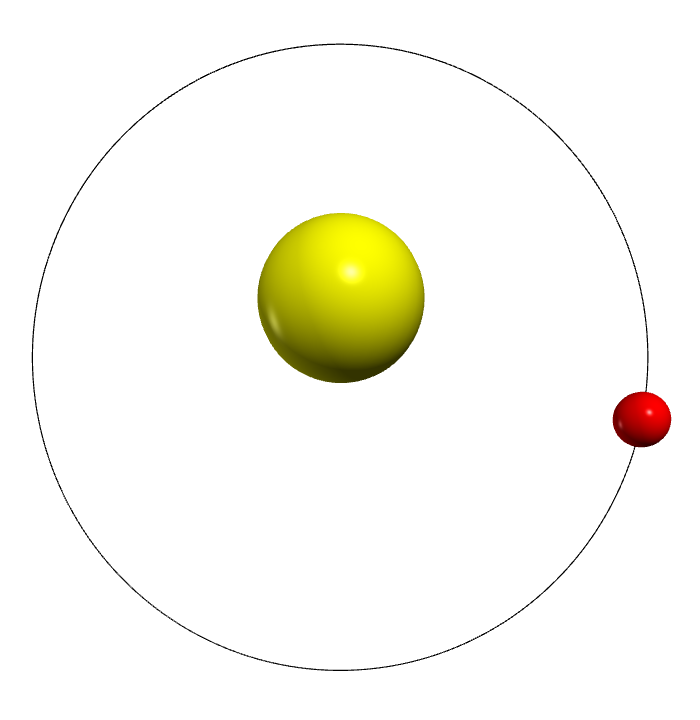
\includegraphics[width=\textwidth]{figs/a0T5dt20.png}
		\caption{\label{fig:MercuryOrbit-a0-small}}
	\end{subfigure}
	\DIFaddFL{~
	}\begin{subfigure}[c]{0.22\textwidth}
		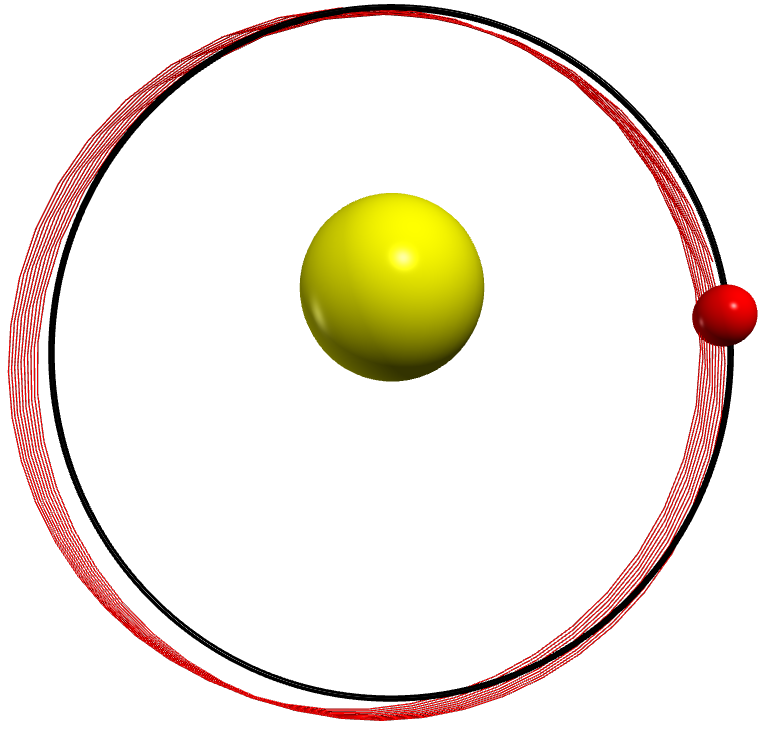
\includegraphics[width=\textwidth]{figs/num-err.png}
		\caption{\label{fig:MercuryOrbit-a0-small-dt-large}}
	\end{subfigure}
	\captionsetup{singlelinecheck=off}
	\caption[]{\label{fig:MercuryOrbit1}
		\DIFaddFL{Different Mercury orbits for the purely Newtonian gravity~(8) and
		 $\Delta t = \Delta t_0  / 20$ for (a) and $\Delta t = \Delta t_0  \times 2$ for (b),
		 where the black line represents the orbit of (a) and the red line is the orbit for the larger time steps.
		The reference time step $\Delta t_0$ is defined via inequality~(7) as explained in the text.
		The images are screenshots of the simulation that is described below (with modified colors).
	}}
\end{figure}
\DIFaddend 

\setcounter{equation}{6 t}
This procedure can only work if $\Delta t$ is sufficiently small.
One way to estimate whether $\Delta t$ is small enough is to verify whether the relation
\begin{equation}
|\vec v(t)| \gg \frac12|\vec a(t)|\Delta t = \frac{1}{2m} |\vec F(\vec r(t)) |\Delta t\
\label{eq:check}
\end{equation}
holds. This follows from Eq.~(1) where the first term that \DIFdelbegin \DIFdel{we }\DIFdelend \DIFaddbegin \DIFadd{was }\DIFaddend neglected reads $(1/2)a(t){(\Delta t)}^2$.
\DIFaddbegin \DIFadd{The impact of the size of $\Delta t$ on the simulation is illustrated in Fig.~\ref{fig:MercuryOrbit1} where
only Newtonian gravity was used. While for the
calculations for the left panel $\Delta t$
is chosen significantly below $\Delta t_0=2m |\vec v(0)| /   |\vec F(\vec r(0)) |$ ($cf.$ }\DIFaddend Eq.~(\DIFaddbegin \DIFadd{\ref{eq:check})), for the
right panel it was chosen twice as large. Accordingly, only the trajectory in the left panel shows the characteristic
feature of a $1/r^2$--force of an ellipse fixed in space. The trajectory in the right panel does not reproduce itself in successive revolutions.
}


\subsection*{Page 19, before section previous 8. Summary}

\DIFaddbegin \section*{\DIFadd{8. Own experiences with the implementation of the course}}

\DIFadd{Work on the subject began with a project work of one of the authors (JH).
The project was presented at the M\"adchen-Gymnasium J\"ulich (a German high school) in 11$^{\rm th}$ grade in 2014.
Based on this study, the course was developed as outlined in Sec.~4 and used in the Sch\"ulerakademie Teilchenphysik in 2015, which aims at high school students from 10$^{\rm th}$ to 13$^{\rm th}$ grade.
This academy is financed by the German Research Society (DFG) as the outreach branch of a research grant focussing on basic research in particle and nuclear physics.
One of the authors (CH) is acting as a Principal Investigator for the outreach activities within this scheme.
The Sch\"ulerakademie Teilchenphysik runs biennially at the Science Center Overbach in J\"ulich for four days and has about 25 participants coming from various parts of Germany.
The academy comprises lectures, a tour to the particle accelerator COSY and the high performance computing facility at the Research Center J\"ulich as well as one full day of practical work.
Given the setting, the participating students are highly motivated and eager to understand.
}

\DIFadd{The course presented in this paper is offered as one out of three hands-on project options.
A lecture to the whole group explaining the basics of numerical simulations laid down some foundations in addition to what is presented in this paper.
Given the positive to enthusiastic feedback we have received from the participants on the course after its first installation in 2015, we decided to make the course a permanent part of the academy.
In 2017 we received similarly positive feedback.
About one half of the participants of each year chose to work on the numerical project --- out of those about one half had previous programming experience.
Most of the participants had already learned about derivatives and vector calculus in school.
}

\DIFadd{The numerical course was allocated for one work day (seven hours) and the students worked in pairs.
Each group worked on a laptop provided by us, where the necessary software was pre-installed.
Four of the authors (IH, CK, CM, JLW) acted as supervisors for the students although not all at the same time. Each instance of the course was supervised by one to three people.
The course was initiated with a brief summary of previously presented methods, motivations and objectives of the simulation.
In the first two hours the students were introduced to \python{} and \vpython{}.
In the following part the students worked with an initial code template (see~[6]) and were motivated to come up with own solutions to fulfill the objectives.
A large part of the material covered during this day is presented in Sec.~4.
With the exception of some younger students, the participants where able to simulate and visualize the motion of mercury including forces from GR.}\@
\DIFadd{Only a few participants started to implement the quantitative extraction of the perihelion motion, uncertainty estimates were not a subject as the time frame was too short.
Once the basic problem was tackled some students deviated from the suggested path and for instance studied the problem with one additional planet or different starting parameters.
This is a very interesting problem by itself for there are parameter ranges where the classical three-body system develops chaotic features.
We encouraged such explorations as well.
We include the additional material in the paper because we want to provide teachers with sufficient material to fill a working group outside the general curriculum running for a longer period than one day.
}


\DIFaddend \end{document}
